\documentclass[fleqn]{article}

\usepackage{mydefs}
\usepackage{notes}
\usepackage{url}
\usepackage{amsmath}
\usepackage{graphicx}
\graphicspath{ {images/} }
\usepackage{verbatim}


\begin{document}
\lecture{Computer Vision}{HW04: Image processing}{CS 670, Fall 2016}

% IF YOU ARE USING THIS .TEX FILE AS A TEMPLATE, PLEASE REPLACE
% "CS 726, Fall 2011" WITH YOUR NAME AND UID.

Hand in via moodle at: \url{https://moodle.umass.edu/course/view.php?id=33024}.
Remember that only PDF submissions are accepted.  We encourage using
\LaTeX\ to produce your writeups.  See \verb+hw00.tex+ for an example
of how to do so.  You can make a \verb+.pdf+ out of the \verb+.tex+ by
running ``\verb+pdflatex hw00.tex+''.

\bee
\i Show that filtering an image with a seperable 2D filter kernel is equivalent to filtering the with two 1D filter kernels.

\vspace{1in}
% ANY LINE BEGINNING "%" IS A COMMENT.  YOU CAN UNCOMMENT THE BELOW
% TEXT AND FILL IN YOUR OWN.
\begin{solution}
Consider any separable filter X with its component filters X1 and X2 as

\[
X = 
\begin{pmatrix}
  x1y1 & x1y2 & x1y3\\
  x2y1 & x2y2 & x2y3\\
  x3y1 & x3y2 & x3y3
\end{pmatrix}
, X1 =
\begin{pmatrix}
  x1\\
  x2\\
  x3
\end{pmatrix}, X2 = 
\begin{pmatrix}
y1 & y2 & y3 
 \end{pmatrix}
\]

Consider any 3X3 image or image patch I as:
\[
I =
\begin{pmatrix}
p11 & p12 & p13\\ 
p21 & p22 & p23\\
p31 & p32 & p33
 \end{pmatrix}
\]

For convolving image I with our 2D filter X we will center the filter at the pixel p22. This will give us the resultant image as
\[
I.X = 
\begin{pmatrix}
x1.y1.p11 & x1.y2.p12 & x1.y3.p13\\ 
x2.y1.p21 & x2.y2.p22 & x2.y3.p23\\
x3.y1.p31 & x3.y2.p32 & x3.y3.p33
 \end{pmatrix}
\]

Now let's look at the result of applying convolution on image I by X1 and then by X2.
Convolving the image I with X1 will give us
\[
I.X1 = 
\begin{pmatrix}
x1.p11 & x1.p12 & x1.p13\\ 
x2.p21 & x2.p22 & x2.p23\\
x3.p31 & x3.p32 & x3.p33
 \end{pmatrix}
\]

and then convolving above result with the X2 will give us
\[
I.X1.X2 = 
\begin{pmatrix}
x1.y1.p11 & x1.y2.p12 & x1.y3.p13\\ 
x2.y1.p21 & x2.y2.p22 & x2.y3.p23\\
x3.y1.p31 & x3.y2.p32 & x3.y3.p33
 \end{pmatrix}
\]
Which is equal to I.X. So filtering an image with a seperable 2D filter kernel is equivalent to filtering the with two 1D filter kernels
\end{solution}
\newpage
\i One way to obtain a Gaussian kernel is to filter a constant kernel with itself many times. Compare this strategy with evaluating a Guassain kernel.
\bee
\i How many repeated filterings do you need to get a reasonable approximation? You need to establish what a reasonable approximation is; You might plot the quality of approximation against the number of repeated convolutions.
\verbatiminput{gaussian_approx.m}

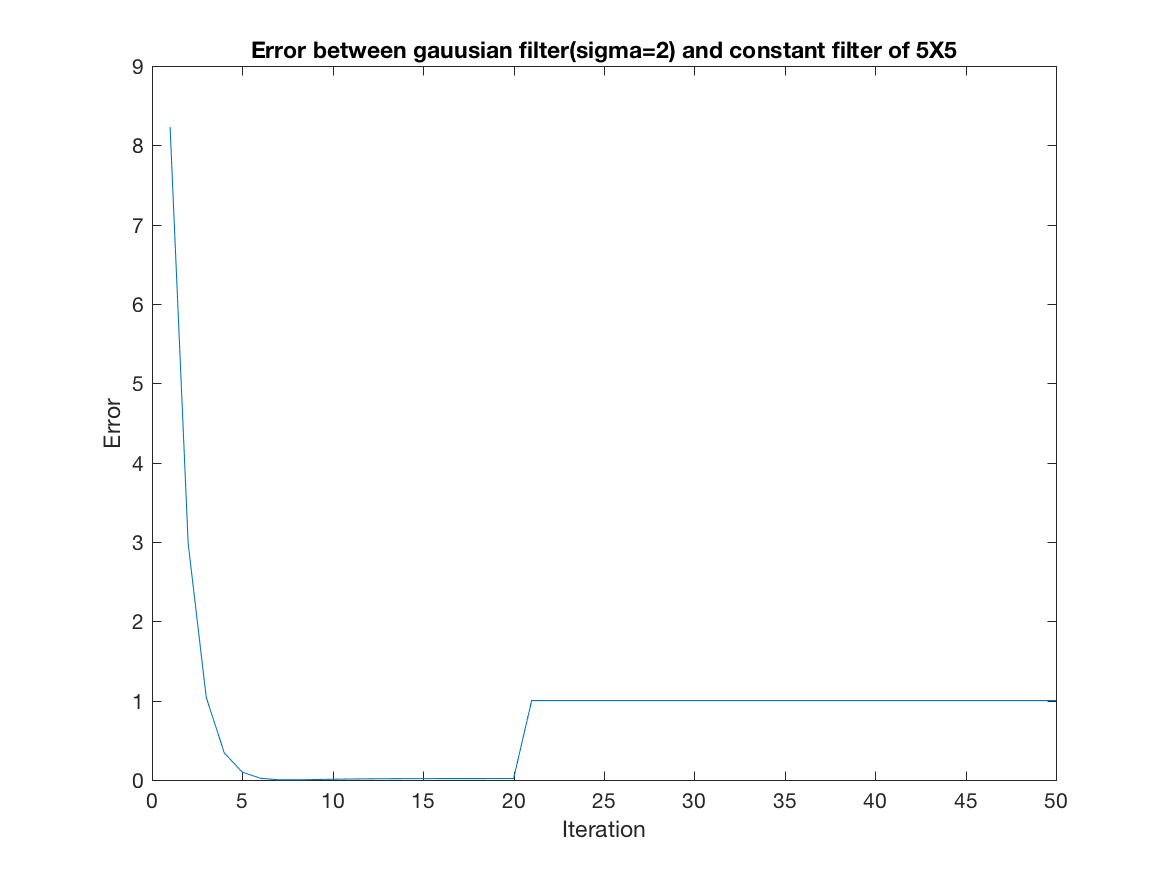
\includegraphics[scale=0.8]{Error5.png}
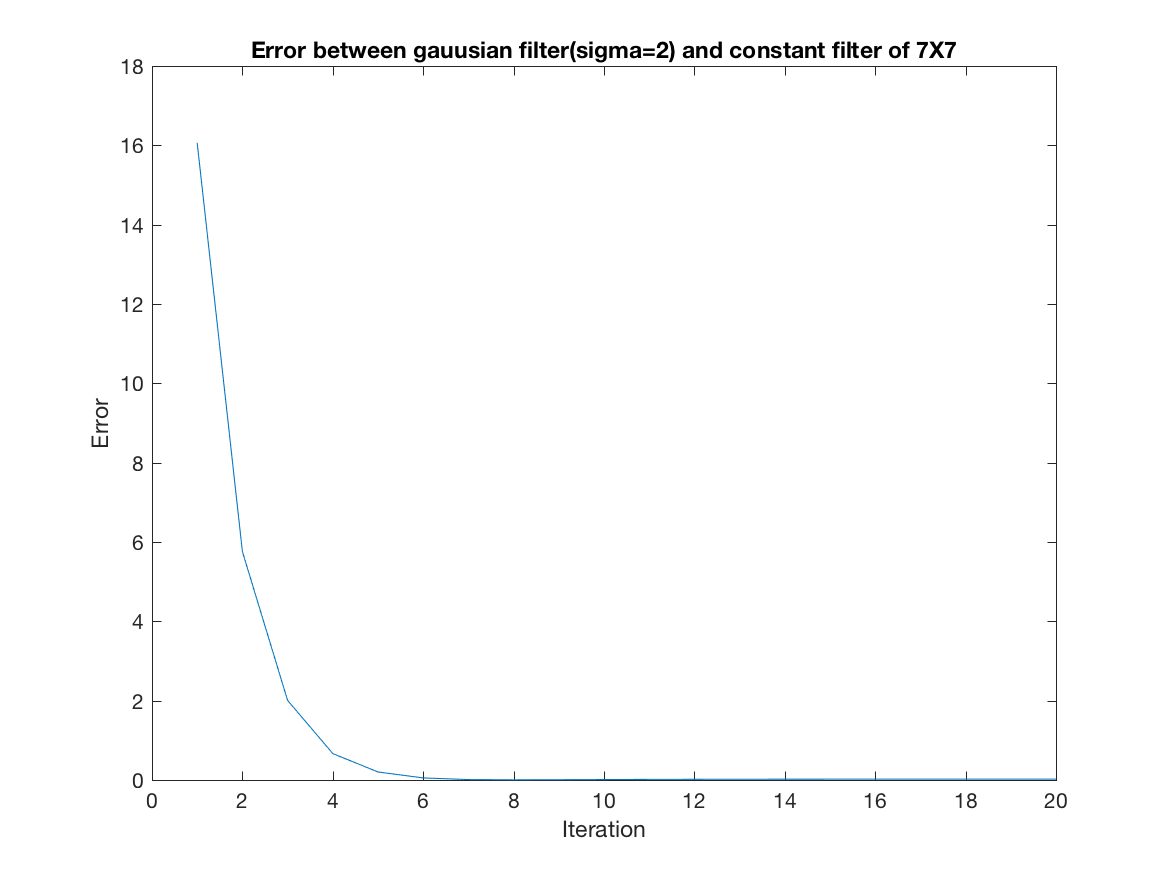
\includegraphics[scale=0.8]{Error7.png}
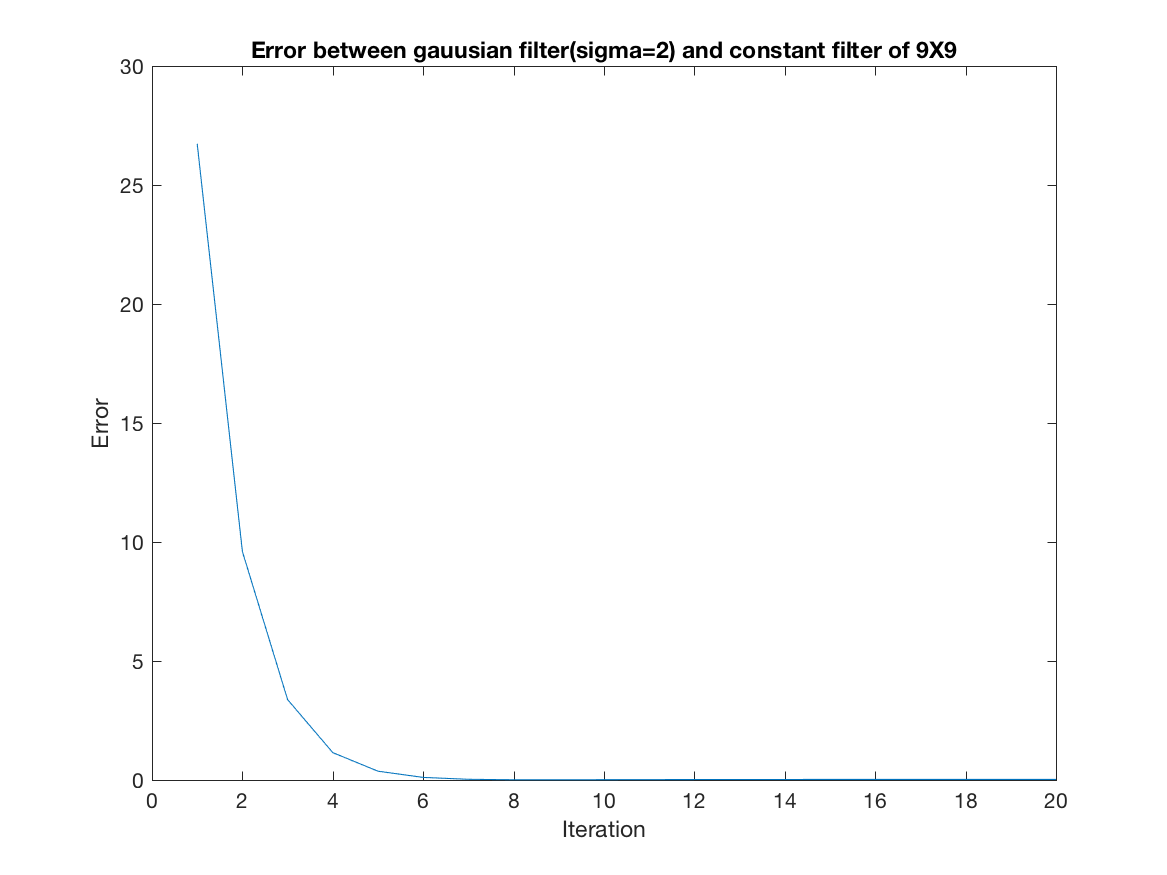
\includegraphics[scale=0.8]{Error9.png}
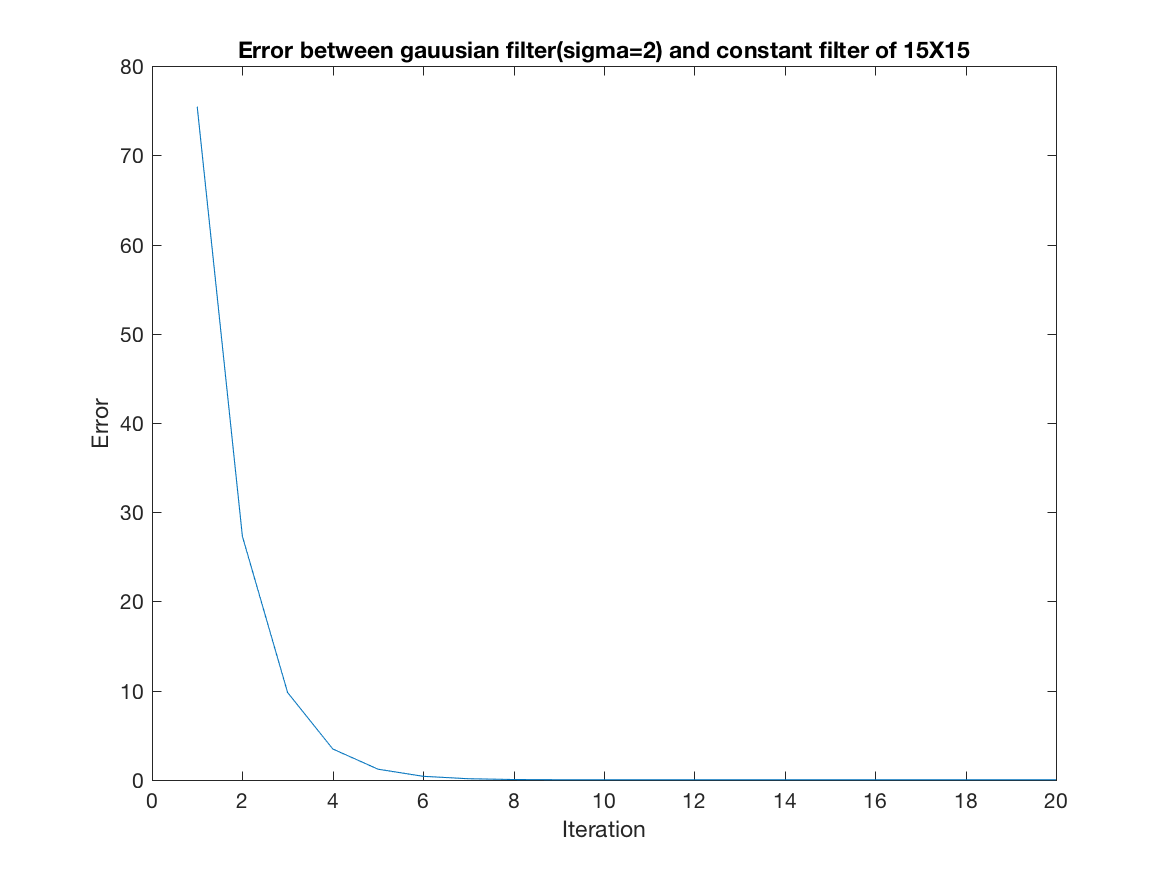
\includegraphics[scale=0.8]{Error15.png}

For different sizes of the filter, error is minimum at the iteration around 6-10. So iterating a constant filter for 6-10(depends on the size of the filter) times with itself gives a close enough approximation of the gaussian filter.

\vspace{1in}
\i Are there any benefits that can be obtained like this?
\vspace{1in}
\ene
\begin{solution}
Generating a gaussian filter dynamically requires complex operations such as exponential terms. If we don't want to do these exponential operations, we can achieve the approximate version by simple operations on a constant filter.
If we can achieve a good approximation in just few iterations, then it can be useful. 
\end{solution}
\ene

\end{document}
